%%% Fiktivní kapitola s ukázkami sazby

\chapter{Introduction to sentiment analysis and existing methods}

\section{Sentiment analysis}
Sentiment analysis (also known as opinion mining) is a type of text analysis focused on detecting polarity (e.g. positive or negative opinion) within text. This chapter serves as an introduction to the field of sentiment analysis and gives an overview of existing tools and current practices.
\subsection{Levels of sentiment analysis}
Liu \cite{liu_2015} describes 3 levels of sentiment analysis:
\begin{itemize}
    \item \textbf{Document level} -- determines the sentiment based on the entire text, which is most useful when the document expresses opinion on a single entity
    \item \textbf{Sentence level} -- classifies each sentence as positive, negative or neutral, mostly used for subjectivity classification  
    \item \textbf{Entity and Aspect level} -- recognizes the different entities described in the text and their aspects and extracts opinions linked with these aspects
    \end{itemize}
Given that the review forms express different opinions on different aspects of a paper, an opinion on a single one of these aspects can span across many sentences, sentiment analysis should therefore be done on an aspect level.
\subsection{Definition of opinion}
In order to explain the task of opinion analysis, we first need to have a definition of an opinion. This is how Liu \cite{liu_2015} defines an opinion:

\begin{quote}
An opinion is a quadruple,\begin{quote} (e, a, s, h, t)\end{quote}where $e$ is the opinion (or sentiment) target entity, $a$ is the aspect of said entity, $s$ is the sentiment about the target, $h$ is the opinion holder and $t$ is the time when the opinion was expressed. 
\end{quote}
For the needs of sentiment analysis in the task of extracting opinions from the final versions of paper reviews, a sufficient definition should be just a tuple (e, s). As reviews sometimes may have more versions than the final one, and because sometimes, a review also may contain an opinion of the author of the reviewed paper (a sentence such as "Although the author believes that his idea is novel, that is not the case" expresses the opinions of two opinion holders -- the author and the reviewer), in future the system may be improved to account for this and therefore use the original quadruple definition of an opinion.
\subsection{Classification of sentiment}

\subsection{Sentiment analysis tasks}

Another thing needing definition is the general way sentiment analysis is done.
\textcite{liu_2015} describes the task of sentiment analysis as a process of six steps, working with:
\begin{enumerate}
    \item entity extraction and categorization
    \item opinion holder extraction and categorization
    \item aspect extraction and categorization
    \item time extraction and standardization
    \item aspect sentiment classification
    \item opinion quintuple generation
\end{enumerate}

 Since conference paper review only describe one entity (the paper) and all opinions should belong to a single person (the reviewer), those parts of the analysis can be left out, as well as time extraction, since that information is not relevant in the generation of visual metaphors. Therefore the steps actually taken in the sentiment analysis of conference paper reviews are these:
 \begin{enumerate}
    \item \textbf{aspect extraction and categorization} -- Extract aspects expressions of the defined review metrics and cluster them based on the metrics they represent
    \item \textbf{aspect sentiment classification} -- Determine whether an opinion on an aspect is positive, negative or neutral and assign it a numeric value describing the polarity of the opinion as well as the strength of the sentiment
    \item \textbf{opinion tuple generation} -- produce the tuples (aspect, sentiment) based on the previous steps
    \end{enumerate}
\section{Sentiment analysis techniques}
\subsection{Machine learning}
Machine learning methods, both supervised and unsupervised, can be used for sentiment analysis. \cite{liu_2015}. For example aspect extraction can be done by Conditional Random Field (CRF), a supervised learning method commonly used in natural language processing \cite{schouten_2016}. Another technique, by Hu and Liu \cite{hu_liu_2015}, which is further explained in section \ref{Aspect Extraction} uses association mining to extract features. However most machine learning methods mostly focus on sentiment analysis on the document level.
 One such technique, which is fairly simple, but often used for simple sentiment analysis is the na\"ive Bayes classifier.
 

   \begin{figure}[htbp!]\centering
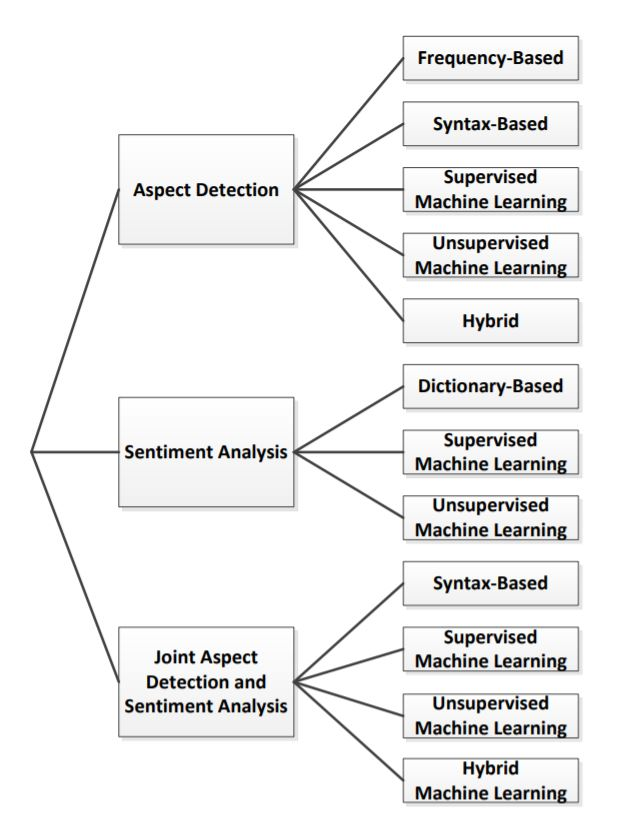
\includegraphics[width=.66\textwidth]{img/taxonomy_om}
      \caption[Taxonomy for aspect-level sentiment analysis]{Taxonomy for aspect-level sentiment analysis \cite{schouten_2016}}\label{img01:taxOM}
    \end{figure}
\subsubsection{The na\"ive Bayes classifier}
\label{sec:NBC}
 Naïve Bayes is a simple machine learning algorithm that utilizes  Bayes rule together with a strong (or na\"ive) assumption that the evidence are conditionally independent, given the hypothesis. \cite{NB}

Therefore the equation for the probability of a hypothesis $H$ given a set of evidence $E_{1},\ldots,E_{K}$, that the na\"ive Bayes classifier is based on is:

$$P\left(H|E_{1},\ldots,E_{K}\right)=\frac{P(H)}{P(E_{1},\ldots,E_{K})}\times\prod_{k=1}^{K}P\left(E_{k}|H\right)
$$

The goal of the classifier is to determine which of the possible hypothesis is the most probable given the evidence.

In the task of sentiment analysis, the different ``classes'' that serve as hypothesis are the different sentiment polarities we try to detect. So we can for example have three different classes -- positive, negative and neutral.

As I already mentioned, when classifying using the na\"ive Bayes algorithm, we look for the hypothesis for which the probability given the evidence is the highest. Therefore we can simplify the equation for $P\left(H|E_{1},\ldots,E_{K}\right)$, leaving the denominator out, because $P(E_{1},\ldots,E_{K}$ will always stay the same for all possible classes/hypothesis:

$$P\left(H|E_{1},\ldots,E_{K}\right)=P(H)\times\prod_{k=1}^{K}P\left(E_{k}|H\right)$$


The evidence are the words contained in the text we want to classify. The text is represented as a bag-of-words, meaning instead of considering the position of each word in the text, we represent it as an unordered set.

When training the na\"ive Bayes classifier we also consider the frequency of each word in each text. We also need a to have each text annotated with its sentiment. The idea behind the bag-of-word approach is depicted on figure \ref{img02:bof}
.
   \begin{figure}[htbp!]\centering
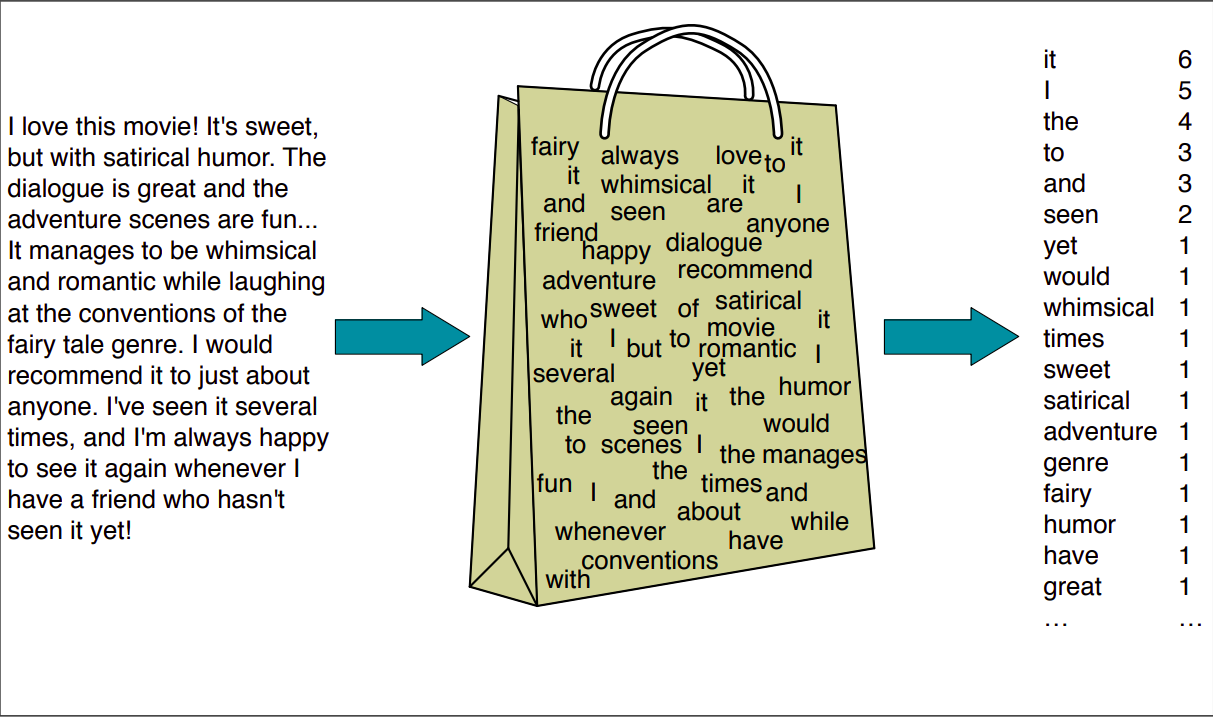
\includegraphics[width=.66\textwidth]{img/bagofwords}
      \caption[Intuition of the multinomial naive Bayes classifier applied to a movie review]{Intuition of the multinomial naive Bayes classifier applied to a movie review \cite{bagofwords}}\label{img02:bof}
    \end{figure}


Then we calculate all the necessary probabilities ($P(c)$ and $P(w_{i}|c)$ or $P(H)$ and $P(E_{k}|H)$ from the original formula) we need for classification of new texts.

The formula for the prior probability of a given class $c$ is:

$$P(c) = \frac{N_{c}}{N}$$

where $N_{c}$ is the number of text belonging to the class $c$ and $N$ is the total amount of texts in the training dataset.

The probability of a word $w_{i}$ occurring in a text with a given class $c$ is:

$$ P(w_{i}|c) = \frac{count(w_{i},c)}{\sum_{w \in V} count(w,c)} $$

where $V$ is the vocabulary, consisting of all words found across all texts, $count(w_{i},c)$ is number of times the word $w_{i}$ appears in documents belonging to class $c$ and the sum of $count(w,c)$ over all words in the vocabulary calculates the sum of all words in all documents of class $c$.

Because the na\"ive Bayes classifier multiplies all evidence likelihoods together, this equation is usually adjusted to account for the fact that some words might never appear in the training set or never appear in conjuction with some class. This makes their probability given a class zero and therefore the probability of said class also zero, independently on all the other words that appeared in the text. This behavior is usually corrected by givin these words non-zero probabilities e.g. using the add-one (Laplace) smoothing\cite{bagofwords}:

$$ P(w_{i}|c) = \frac{count(w_{i},c) + 1}{(\sum_{w \in V} count(w,c)) + |V|} $$

To give a clear example of an application of the na\"ive Bayes classifier on the task of sentiment analysis, here is how we would calculate the probability of a sentence ``This phone is great.'' being positive:

\begin{align*}
P(positive|``this",`` phone ",``is",``great")&=\\ 
&=P(``this"|positive) \\
&\times P(``phone"|positive) \\
&\times P(``is"|positive) \\
&\times P(``great"|positive)\\
&\times P(positive)
\end{align*}

\subsection{Dictionary-based Approaches}
The biggest indicators of sentiment in a text are sentiment words (also called opinion words). These words, often adjectives or adverbs, help to detect the expression of sentiment as well as its polarity. For example words such as \textit{great},\textit{amazing} or \textit{good} indicate a positive sentiment, on the other hand words like \textit{terrible}, \textit{awful} or \textit{bad} express negative feelings. \cite{liu_2015}
  
  
  In order to obtain a sentiment lexicon, Liu \cite{liu_2015} mentions 3 main approaches:
  \begin{itemize}
      \item \textbf{manual approach} -- is usually combined with automated methods because of its labor intensity
      \item \textbf{dictionary-based approach} -- usually uses a list of a small number of sentiment words as a seed and then generates the dictionary through tools such as \textcite{wordnet}   by integrating their synonyms or antonyms
      \item \textbf{corpus-based approach} -- the aim is to create a sentiment lexicon for a specific domain, for example by using a seed of sentiment words and then including other words in the lexicon by searching the sentences for conjoined adjectives, where one is already known as a sentiment word
  \end{itemize}
  There also are already compiled dictionaries of sentiment words, such as SentiWordNet \footnote{\url{https://github.com/aesuli/sentiwordnet}}, which assigns to each word both a positive score and a negative score (on a scale from 0 to 1) and allows to obtain an objectivity score based on the two. SentiWords \footnote{\url{https://hlt-nlp.fbk.eu/technologies/sentiwords}} or SenticNet \footnote{\url{https://sentic.net/}}, assign to each word they contain a sentiment score between -1 (extremely negative) and +1 (extremely positive).
  
  Lexicon-based approaches of sentiment analysis, as the name suggests, utilize lexicons of sentiment words as well as other constructs like sentiment shifters, but-clauses and other words or phrases that affect sentiment.
\subsubsection{Sentimentr}
One tool that utilizes a lexicon-based method for sentiment analysis is sentimentr.

 As explained in the sentimentr documentation ``sentimentr attempts to take into account valence shifters (i.e., negators, amplifiers (intensifiers), de-amplifiers (downtoners), and adversative conjunctions) while maintaining speed. Simply put, sentimentr is an augmented dictionary lookup.'' \cite{sentimentr}.
 
The way sentimentr works is that instead of simply comparing the words in sentence with the sentiment lexicon and judging the sentiment of a sentence based on, say, the sum of polarities of sentiment words found within it, it also adjusts the polarity of each sentiment word based on sentiment shifters found in the proximity of that word. The influence of different valence shifters is as follows:

\paragraph{Negators.} Negators are words such as ``no, not, never''. The influence of negators on the polarity of a sentiment word is simple -- if the number of negators in the left and right context of a sentiment word is even the polarity stays the same, however if the number is odd, the polarity is negated (so a word with originally negative polarity becomes positive and vice versa)

\paragraph{Amplifiers.} Amplifiers are words like ``especially, major, significantly''. As the name suggests they increase (amplify) the polarity of a sentiment word. There is however one exception to this rule -- if the number of negators in the context of a sentiment words is odd, the influence of amplifiers is negated, aka they start working as the de-amplifiers described bellow.

\paragraph{De-amplifiers} De-amplifiers, like ``slightly, somewhat sort of'' etc. work analogously to amplifiers, except they decrease the polarity of a sentiment word instead of increasing it.

\paragraph{Adversative conjuction} Adversative conjuctions are perhaps the most complex of the valence shifters. These are words such as ``bur, however, albeit''. The relative position of an adversative conjuction to the sentiment word plays an important role when determining its influence. If the conjuction comes before the sentiment word it increases its polarity, however if it comes after it decreases it. According to the sentimentr documentation ''This corresponds to the belief that an adversative conjunction makes the next clause of greater values while lowering the value placed on the prior clause.''. \cite{sentimentr}


The final sentiment score of a sentence is calculated as follows:

$$\textrm{sentiment}(s) = \frac{\sum_{w_{i} \in Pol} sentiment(w_{i})}{\sqrt{|w_{i}|}}$$

where $s$ is the sentence, $w_{i}$ is the $i$-th word of the sentence, $Pol$ is a set o polar/sentiment words in the sentence, $sentiment(w_{i})$ is the calculated sentiment of $w_{i}$ and $|w_{i}|$ is the length of the sentence.

The sentiment of a word adjusted by the valence shifters is calculated as:

\subsubsection{A Holistic Lexicon-Based Approach} 
Another lexicon-based approach is one called ``a holistic lexicon-based approach''.\cite{ding_hu_liu} This one, contrary to the \textit{sentimentr} method described above which determines the sentiment on a sentence level, focuses on aspect-based sentiment analysis. 

The basic algorithm finds all words or phrases describing features in a sentence as well as opinion (or sentiment) words. Then, for each feature in the sentence, its sentiment score is calculated using the polarity of the opinion words and their distance in the sentence from the feature expression using the following function:
$$
\textrm{score}(f) = \frac{\sum_{w_{i} : w_{i} \in s \wedge w_{i} \in V}w_{i}.SO}{dis(w_{i},f)}
$$

where:
\begin{itemize}
\item $w_{i}$ is an opinion word
\item $V$ is the set of all opinion words
\item $s$ is the sentence that contains the feature $f$
\item  $dis(w_{i} , f)$ is the distance between feature $f$ and
opinion word $w_{i}$ in the sentence $s$
\item $w i .SO$ is the semantic orientation of the word $w_{i}$
\end{itemize}
Then ``If the final score is positive, then the opinion on the feature in
the sentence s is positive. If the final score is negative, then
the opinion on the feature is negative. It is neutral otherwise.''\cite{ding_hu_liu}.

The algorithm is also extended to deal with negation (by negating the polarity of a sentiment word which follows after a negation word), ``but'' clauses (by first trying to determine the sentiment of an opinion word within the ``but'' clause using the basic algorithm and if the sentiment score is zero it assigns the negation of the clause before ``but''). Then it has these three rules for dealing with context-dependent opinion words:
\begin{itemize}
\item \textbf{Intra-sentence conjunction rule} -- this rule is based on the idea that ``a sentence only expresses one opinion
orientation unless there is a `but' word which changes the
direction.''\cite{ding_hu_liu}. Therefore if the orientation of one opinion word depends on the context but there is another opinion word in the sentence for which the orientation is known and the clauses containing the two opinion words are connected by a conjunction such as ``and'', we can assign that orientation to the context-dependent orientation word as well.
\item \textbf{Pseudo intra-sentence conjunction rule} -- this rule applies to sentences without an explicit conjunction, but otherwise works the similarly to the previous rule
\item \textbf{Inter-sentence conjunction rule} -- if the opinion orientation is still undetermined after the application of previous rules, the inter-sentence conjunction rule helps assign the orientation using the context of the surrounding sentences. According to the authors ``The idea is that people usually express the same
opinion (positive or negative) across sentences unless there is
an indication of opinion change using words such as `but' and
`however'.''\cite{ding_hu_liu}.
\end{itemize}
\section{Aspect extraction}
\subsection{Frequency extraction}
In order to extract aspect expressions, Hu and Liu \cite{hu_liu_2015} propose using a Part Of Speech (POS) tagger to identify nouns and noun phrases as possible aspect expression candidates. Then they use a simplified Apriori algorithm to calculate frequency of these candidates and finally keep only the ones that are frequent enough. 
  
  Their reasoning is that the vocabulary people use when commenting on an entity converges, so the frequently co-occurring sets of terms should represent the important aspects.
\subsection{Taxonomy based extraction}
\label{sec:taxonomy}
 Another approach, by Carenini\cite{carenini_2005}, uses user's prior knowledge of the domain to build a hierarchy of features. Their technique uses the previously mentioned unsupervised learning technique developed by Hu and Liu and adds user-defined features and similarity matching in order to eliminate redundancy  and to generate a set of features in an organized way, reflecting hierarchical relationships between them.
The way their method works is that first a set of ``crude features'' is generated by Hu and Liu's method.

Then  the WordNet lexical database is used to perform similarity matching between the user-defined taxonomy of features and the crude features. Only the crude features that are similar enough to the features already included in the taxonomy are then further used. 

Finally the newly discovered feature candidates which passed the similarity matching are inspected by a user and if the user considers these candidates valid feature expression, they are added to the final taxonomy.
\subsection{Patterns for aspect extraction}
A very different technique for aspect extraction is described by Asghar et al.\cite{asghar_2019}. Their opinion mining framework comprises of a set of heuristic patterns for extraction of aspects as well as sentiments or opinions. 

In order to get the pairs of aspects and the related sentiments, the reviews first go through a preprocessing phase, part of which is POS tagging. After that, the POS tagged sentences are matched against a set of patterns. Each pattern is a sequence of POS tags, so in order to get a match against one of them, the sentence must contain that sequence of tags as well. 

The part of the pattern which is a noun, noun phrase or a verb is then considered to be a candidate term for an aspect while mostly adjectives and adverbs represent the expression of sentiment.
